\documentclass[11pt]{article}

\usepackage[a4paper,margin=1in]{geometry}
\usepackage[T1]{fontenc}
\usepackage[utf8]{inputenc}
\usepackage{lmodern}
\usepackage[nopatch=footnote]{microtype}
\usepackage{amsmath,amssymb}
\usepackage{bm}
\usepackage{booktabs}
\usepackage{array}
\usepackage{enumitem}
\usepackage{graphicx}
\usepackage{hyperref}
\usepackage{xurl}
\usepackage{setspace}
\usepackage[numbers,sort&compress]{natbib}
\newcolumntype{L}[1]{>{\raggedright\arraybackslash}p{#1}}
\onehalfspacing

\newcommand{\dd}{\mathrm{d}}
\newcommand{\pp}{\partial}
\newcommand{\Rey}{\mathit{Re}}
\newcommand{\Ma}{\mathit{Ma}}
\renewcommand{\Pr}{\mathit{Pr}}
\newcommand{\bq}{\mathbf{q}}
\newcommand{\bqp}{\mathbf{q}'}
\newcommand{\bqbar}{\bar{\mathbf{q}}}
\newcommand{\bx}{\mathbf{x}}
\newcommand{\bA}{\mathbf{A}}
\newcommand{\bB}{\mathbf{B}}
\newcommand{\bC}{\mathbf{C}}
\newcommand{\bH}{\mathbf{H}}
\newcommand{\bI}{\mathbf{I}}
\newcommand{\bL}{\mathbf{L}}
\newcommand{\bM}{\mathbf{M}}
\newcommand{\bF}{\mathbf{F}}
\newcommand{\bP}{\mathbf{P}}
\newcommand{\bR}{\mathbf{R}}
\newcommand{\bS}{\mathbf{S}}
\newcommand{\bW}{\mathbf{W}}
\newcommand{\bv}{\mathbf{v}}
\newcommand{\by}{\mathbf{y}}
\newcommand{\bb}{\mathbf{b}}
\newcommand{\br}{\mathbf{r}}
\newcommand{\KSP}{\texttt{KSP}}
\newcommand{\PC}{\texttt{PC}}

\title{\texttt{linstab2d}: compressible stability and resolvent analysis with PETSc/SLEPc}
\author{Gabriel Hamada \and Ricardo Frantz}
\date{}

\usepackage{tikz}
\usetikzlibrary{arrows.meta,positioning,shapes.geometric,calc,fit}
\begin{document}
\maketitle

\begin{abstract}
This paper presents \texttt{linstab2d}, an open-source Python implementation of compressible linear stability and resolvent analysis that couples the mathematical framework of Martini \& Schmidt (2024) with PETSc/SLEPc sparse solvers.
We document the full formulation implemented in the code: the five-variable compressible linearized Navier--Stokes equations (LNSE) for the primitive state vector $\bqp=[\rho',u',v',w',T']^\top$, discretized with summation-by-parts (SBP) finite differences on curvilinear grids.
The mathematical documentation covers the complete operator assembly --- including Sutherland viscosity, the spatial companion linearization for the quadratic eigenvalue problem, the Chu energy norm for compressible disturbance energy, Floquet decomposition for streamwise-periodic base flows, and high-order implicit Pad\'e-type filtering --- at the level of detail needed to reproduce the implementation.
The analysis framework includes temporal and spatial eigenvalue problems and resolvent analysis.
Two solver strategies address the dominant computational cost --- repeated sparse linear solves of large shifted non-Hermitian systems: a robust MUMPS sparse-direct baseline and a scalable PETSc iterative path with additive Schwarz preconditioning.
The paper defines validation and benchmark protocols for agreement with the MATLAB reference and for large sparse runs.
Quantitative accuracy and performance claims are restricted to the cases whose tables and figures are explicitly populated in Section~\ref{sec:results}.
The implementation is released as open-source Python with no MATLAB dependency.
\end{abstract}

\noindent\textbf{Keywords:} compressible stability; resolvent analysis; linearized Navier--Stokes; summation-by-parts finite differences; Chu energy norm; PETSc; SLEPc; MUMPS

%======================================================================
\section{Introduction}
\label{sec:intro}
%======================================================================

Linear stability and resolvent analysis are cornerstones of modern transition prediction and turbulence modeling in compressible flows.
The mathematical foundations --- eigenvalue decomposition for modal instabilities and input--output (resolvent) analysis for nonmodal amplification --- are well established \cite{schmid2001stability,schmid2007nonmodal,trefethen1993hydrodynamic}.
Their application to two-dimensional and global configurations has been reviewed by Theofilis \cite{theofilis2011global}, while Taira et al.\ \cite{taira2017modal,taira2020modal} provide a broader perspective on modal analysis techniques in fluid mechanics, including connections to data-driven methods.

A central development in this area is the resolvent framework introduced by McKeon \& Sharma \cite{mckeon2010critical} and further developed by Towne et al.\ \cite{towne2018spectral}, which recasts the linearized dynamics as a transfer operator between forcing and response.
This viewpoint unifies classical stability theory with nonmodal growth and has become a standard tool for analyzing turbulent flows.
For compressible flows specifically, the resolvent formulation requires careful treatment of the energy inner product, where the Chu norm \cite{chu1965energy,hanifi1996compressible} provides a physically meaningful measure of disturbance energy.

The MATLAB implementation of Martini \& Schmidt \cite{martini2024} (hereafter M\&S) provides a well-documented reference for compressible stability and resolvent analysis on structured grids, including curvilinear coordinate transformations, summation-by-parts (SBP) finite-difference operators, and implicit spatial filtering.
Several other tools address related problems: \texttt{resolvent4py} \cite{padovan2025resolvent4py} provides a Python framework for resolvent and modal decomposition, while the one-way Navier--Stokes (OWNS) approach \cite{towne2022efficient} offers an efficient alternative for convectively dominated flows.

The contribution of the present work is twofold.
First, we provide a complete open-source Python implementation of the M\&S mathematical framework, including elements not commonly documented in detail: the full five-variable compressible LNSE with Sutherland viscosity, the spatial eigenvalue companion linearization, Floquet-shifted operators for streamwise-periodic flows, the Chu energy norm in discretized form, and high-order implicit Pad\'e-type filtering.
Second, we couple this formulation to PETSc/SLEPc \cite{balay2025petsc,hernandez2005slepc} for transparent control of sparse linear algebra, offering both a robust MUMPS direct-solve baseline \cite{amestoy2001mumps} and a scalable iterative path \cite{saad2003iterative,benzi2002preconditioning} for large-DOF regimes.
A comprehensive review of Krylov methods for large-scale stability and resolvent computations in fluid dynamics is given by Frantz et al.\ \cite{frantz2023krylov}; the companion library \texttt{LightKrylov} \cite{kern2026lightkrylov} provides a modern Fortran implementation of these techniques.

The remainder of this paper is organized as follows.
Section~\ref{sec:equations} presents the governing equations and analysis framework.
Section~\ref{sec:discretization} details the numerical discretization, including SBP operators, curvilinear mappings, boundary treatment, and spatial filtering.
Section~\ref{sec:solvers} describes the PETSc/SLEPc solver architecture.
Section~\ref{sec:results} presents validation and performance results.
Section~\ref{sec:discussion} discusses trade-offs and practical guidance, and Section~\ref{sec:conclusions} concludes.

%======================================================================
\section{Governing equations and analysis framework}
\label{sec:equations}
%======================================================================

%----------------------------------------------------------------------
\subsection{Compressible linearized Navier--Stokes equations}
\label{sec:lnse}
%----------------------------------------------------------------------

We consider the compressible Navier--Stokes equations for a calorically perfect gas, linearized about a steady base flow $\bqbar(\bx)$.
The flow state is decomposed as
\begin{equation}
  \bq(\bx,t) = \bqbar(\bx) + \epsilon\,\bqp(\bx,t),
  \qquad 0 < \epsilon \ll 1,
\end{equation}
where the perturbation state vector in primitive variables is
\begin{equation}
  \bqp = [\rho',\, u',\, v',\, w',\, T']^\top.
  \label{eq:state_vector}
\end{equation}
Here $\rho$ is density, $(u,v,w)$ are the velocity components in the $(x,y,z)$ directions, and $T$ is temperature.

All quantities are non-dimensionalized by a reference length $L^*$, velocity $U^*$, density $\rho^*$, and temperature $T^*$, yielding three governing parameters: the Reynolds number $\Rey = \rho^* U^* L^* / \mu^*$, the Mach number $\Ma = U^* / a^*$ (where $a^* = \sqrt{\gamma R_g T^*}$ is the reference sound speed), and the Prandtl number $\Pr = \mu^* c_p / \kappa^*$.
The equation of state for a perfect gas gives the non-dimensional pressure as
\begin{equation}
  p = \frac{\rho\, T}{\gamma\, \Ma^2}.
  \label{eq:eos}
\end{equation}

The dynamic viscosity follows Sutherland's law:
\begin{equation}
  \mu(T) = \mu_{\mathrm{ref}}\,
  \frac{T_{\mathrm{ref}} + S_1}{T + S_1}
  \left(\frac{T}{T_{\mathrm{ref}}}\right)^{3/2},
  \qquad S_1 = \frac{110.4\;\mathrm{K}}{T^*},
  \label{eq:sutherland}
\end{equation}
Here $T_{\mathrm{ref}}=T_{\mathrm{ref}}^*/T^*$ is the nondimensional Sutherland reference temperature, and $\mu_{\mathrm{ref}}=\mu(T_{\mathrm{ref}}^*)/\mu^*$ is the corresponding nondimensional reference viscosity. If the nondimensionalization uses $T^*=T_{\mathrm{ref}}^*$ and $\mu^*=\mu(T_{\mathrm{ref}}^*)$, then $T_{\mathrm{ref}}=1$ and $\mu_{\mathrm{ref}}=1$.
The bulk viscosity follows the Stokes hypothesis, $\lambda = -\tfrac{2}{3}\mu$, and thermal conductivity is determined by $\Pr$.

Following M\&S \cite{martini2024}, the linearized system is written in matrix form as
\begin{equation}
  \bM\,\frac{\pp\bqp}{\pp t}
  = \left(
      \bA_0
    + \bA_x\,D_x
    + \bA_y\,D_y
    + \bA_{xx}\,D_{xx}
    + \bA_{yy}\,D_{yy}
    + \bA_{xy}\,D_{xy}
  \right)\bqp,
  \label{eq:lnse_matrix}
\end{equation}
where $D_x$, $D_y$, $D_{xx}$, $D_{yy}$, and $D_{xy}$ denote the first and second partial derivative operators, and the $5\times5$ coefficient matrices $\bA_k$ depend on the base-flow variables and their gradients.
The matrix $\bM$ accounts for the density weighting of the primitive-variable momentum and energy equations; for Cartesian two-dimensional configurations it reduces to $\bM = \mathrm{diag}(1,\bar\rho,\bar\rho,\bar\rho,\bar\rho)$, while for axisymmetric flows it is a lower-triangular matrix that additionally performs the conservative-to-primitive variable transformation.
The explicit expressions for $\bA_k$ are given in M\&S \cite{martini2024}; we adopt their notation throughout.
The original coefficient matrices were derived using computer algebra (Mathematica) by Martini \& Schmidt; the present Python implementation was translated from their released MATLAB code.
To guard against errors propagated through this derivation chain (Mathematica $\to$ MATLAB $\to$ Python), we verify the assembled operator independently using two complementary approaches described in~\S\ref{sec:linearization_verification}: symbolic re-derivation with SymPy and a complex-step Jacobian check against the full nonlinear residual.

Key physics encoded in these matrices includes the linearized convection, pressure--density coupling through the equation of state~\eqref{eq:eos}, viscous dissipation with the Stokes hypothesis, Sutherland viscosity derivatives (up to second order), and Fourier heat conduction.

\paragraph{Spanwise Fourier decomposition.}
The spanwise ($z$) direction is assumed homogeneous, so perturbations are decomposed into Fourier modes:
\begin{equation}
  \bqp(x,y,z,t) = \hat{\bq}(x,y,t)\,\mathrm{e}^{\mathrm{i} k_z z},
  \label{eq:spanwise_fourier}
\end{equation}
where $k_z$ is the spanwise wavenumber.
Under this ansatz, the $z$-derivative operators become algebraic multiplications ($D_z \to \mathrm{i}k_z$, $D_{zz} \to -k_z^2$), reducing the three-dimensional problem to a two-dimensional one parameterized by $k_z$.
Setting $k_z = 0$ recovers the purely two-dimensional case.

\paragraph{Axisymmetric formulation.}
For axisymmetric base flows, the coordinates $(x,y,z)$ are interpreted as $(x,r,\theta)$, and the azimuthal direction is decomposed into Fourier modes with integer azimuthal wavenumber $m$:
$\bqp(x,r,\theta,t) = \hat{\bq}(x,r,t)\,\mathrm{e}^{\mathrm{i} m\theta}$.
The coefficient matrices $\bA_k$ then include the additional metric terms $1/r$ arising from cylindrical geometry, and the matrix $\bM$ becomes lower-triangular to perform the conservative-to-primitive transformation.
The quadrature weight matrix $\bW_\Omega$ includes the radial coordinate~$r$ so that inner products integrate over the physical volume element $r\,\dd r\,\dd x$.

%----------------------------------------------------------------------
\subsection{Temporal stability analysis}
\label{sec:temporal}
%----------------------------------------------------------------------

Temporal stability analysis seeks the complex frequencies $\omega$ at which the linearized system admits exponentially growing or decaying solutions.
With the normal-mode ansatz $\bqp(\bx,t) = \hat{\bq}(\bx)\,\mathrm{e}^{-\mathrm{i}\omega t}$, substitution into~\eqref{eq:lnse_matrix} yields the generalized eigenvalue problem
\begin{equation}
  \bL\,\hat{\bq} = \lambda\,\bM\,\hat{\bq},
  \qquad \lambda = -\mathrm{i}\omega,
  \label{eq:gevp}
\end{equation}
where $\bL$ is the spatially discretized LNSE operator and $\bM$ is the discrete mass/conversion matrix.
In the implementation, all factors of $\mathrm{i}$ are confined to the frequency-domain EVP; after left-multiplication by $\bM^{-1}$, the evolution operator is solved in the convention induced by $\bqp(\bx,t)=\hat{\bq}(\bx)\,\mathrm{e}^{-\mathrm{i}\omega t}$.
Consequently, \emph{temporally unstable modes have} $\mathrm{Im}(\omega) > 0$, and the phase speed is $c = \mathrm{Re}(\omega)/\alpha$.

For targeted extraction of eigenvalues near a shift $\sigma$, the shift-invert spectral transformation is used:
\begin{equation}
  (\bL - \sigma\bM)^{-1}\bM\,\bv = \mu\,\bv,
  \qquad \mu = \frac{1}{\lambda - \sigma}.
  \label{eq:shift_invert}
\end{equation}
Each Krylov iteration of the outer SLEPc eigensolver therefore requires one inner sparse linear solve with the shifted matrix $(\bL - \sigma\bM)$, so the quality of the inner solver directly governs the overall computation \cite{frantz2023krylov}.

\paragraph{Adjoint eigenvalues.}
The adjoint operator in the $\bW$-weighted inner product is
\begin{equation}
  \bL^+_{\bW} = \bW^{-1}\bL^H\bW,
  \label{eq:adjoint_op}
\end{equation}
where $\bW$ is the diagonal energy-norm weight matrix defined in~\S\ref{sec:resolvent}.
Adjoint eigenvectors are normalized so that $\bv^H\bW\bv = 1$ (where $\bW$ is real-valued and diagonal).

%----------------------------------------------------------------------
\subsection{Spatial stability analysis}
\label{sec:spatial}
%----------------------------------------------------------------------

Spatial stability analysis seeks the complex streamwise wavenumber $\alpha$ for prescribed real frequency $\omega$.
Under the ansatz $\mathrm{e}^{\mathrm{i}\alpha x}$, downstream spatial growth corresponds to $\mathrm{Im}(\alpha)<0$.
Because the LNSE operator~\eqref{eq:lnse_matrix} depends quadratically on $\alpha$ through the Floquet-shifted derivatives (see~\S\ref{sec:floquet}), and the temporal term contributes an additional $\mathrm{i}\omega\bI$, the resulting eigenvalue problem is a quadratic eigenvalue problem (QEP):
\begin{equation}
  (\bR_0 + \mathrm{i}\omega\bI + \alpha\,\bR_1 + \alpha^2\,\bR_2)\,\hat{\bq} = \bm{0},
  \label{eq:qep}
\end{equation}
where the matrices $\bR_0$, $\bR_1$, and $\bR_2$ are reconstructed from three operator evaluations:
\[
  \bR_0=\bA(0),\qquad
  \bR_1=\frac{\bA(\Delta\alpha)-\bA(-\Delta\alpha)}{2\Delta\alpha},\qquad
  \bR_2=\frac{\bA(\Delta\alpha)-2\bA(0)+\bA(-\Delta\alpha)}{2\Delta\alpha^2},
\]
with the value of $\Delta\alpha$ reported for each run \cite{malik1990numerical}.

The QEP~\eqref{eq:qep} is linearized to a generalized eigenvalue problem of doubled dimension via the companion form.
Defining the frequency-free matrix $\bL_c$ and the frequency-dependent matrix $\bL_{\omega,c}$,
\begin{equation}
  \bL_c =
  \begin{bmatrix}
    \bm{0} & \bI \\
    -\bR_0 & \bm{0}
  \end{bmatrix},
  \qquad
  \bL_{\omega,c} =
  \begin{bmatrix}
    \bm{0} & \bm{0} \\
    -\mathrm{i}\bI & \bm{0}
  \end{bmatrix},
  \qquad
  \bR_c =
  \begin{bmatrix}
    \bI & \bm{0} \\
    \bR_1 & \bR_2
  \end{bmatrix},
  \label{eq:companion_matrices}
\end{equation}
the spatial EVP reads
\begin{equation}
  (\bL_c + \omega\,\bL_{\omega,c})\,\bv = \alpha\,\bR_c\,\bv,
  \qquad
  \bv = \begin{bmatrix} \hat{\bq} \\ \alpha\hat{\bq} \end{bmatrix},
  \label{eq:companion}
\end{equation}
which is a $2n\times 2n$ generalized non-Hermitian eigenvalue problem (GNHEP) solved using SLEPc with shift-invert and MUMPS.

%----------------------------------------------------------------------
\subsection{Resolvent analysis}
\label{sec:resolvent}
%----------------------------------------------------------------------

Resolvent analysis characterizes the amplification between harmonic forcing $\hat{\mathbf{f}}$ and response $\hat{\bq}$ at angular frequency $\omega_f$.
The transfer (resolvent) operator is
\begin{equation}
  \bH(\omega_f) = \bC_{\mathrm{out}}\,(\bL - \mathrm{i}\omega_f\bI)^{-1}\,\bB_{\mathrm{in}},
  \label{eq:resolvent_op}
\end{equation}
where $\bB_{\mathrm{in}}$ and $\bC_{\mathrm{out}}$ are input and output restriction operators that select which state-vector components participate as forcing and response, respectively.
In the default (full-state) configuration, $\bB_{\mathrm{in}} = \bC_{\mathrm{out}} = \bI$, so all five primitive variables are both forced and observed; sub-selecting components (e.g., forcing only the momentum equations) is achieved by replacing $\bB_{\mathrm{in}}$ or $\bC_{\mathrm{out}}$ with rectangular Boolean projection matrices.
In the implementation convention used here, the assembled operator $\bL$ already includes left multiplication by the inverse conversion matrix from~\eqref{eq:lnse_matrix}; therefore the effective resolvent mass matrix is the identity, giving $\bL_\omega = \bL - \mathrm{i}\omega_f\bI$.
The optimal gains $\sigma_j$ and the corresponding forcing--response mode pairs are obtained from the singular value decomposition (SVD) of $\bH$ in an energy-weighted inner product.

The compressible disturbance energy is measured using the Chu norm \cite{chu1965energy}, which in non-dimensional primitive variables reads
\begin{equation}
  E = \frac{1}{2}\int_\Omega
  \left[
    \frac{\bar{T}}{\bar{\rho}\,\gamma\,\Ma^2}\,|\rho'|^2
  + \bar{\rho}\,(|u'|^2 + |v'|^2 + |w'|^2)
  + \frac{\bar{\rho}}{\gamma(\gamma-1)\bar{T}\,\Ma^2}\,|T'|^2
  \right]\dd\Omega.
  \label{eq:chu_norm}
\end{equation}
The corresponding diagonal weight matrix $\bW \in \mathbb{R}^{5N\times 5N}$ has blocks
\begin{equation}
  \bW = \frac{1}{2}\,\mathrm{diag}\!\left(
    \frac{\bar{T}}{\bar{\rho}\,\gamma\,\Ma^2}\,\bW_\Omega,\;
    \bar{\rho}\,\bW_\Omega,\;
    \bar{\rho}\,\bW_\Omega,\;
    \bar{\rho}\,\bW_\Omega,\;
    \frac{\bar{\rho}}{\gamma(\gamma-1)\bar{T}\,\Ma^2}\,\bW_\Omega
  \right),
  \label{eq:W_diag}
\end{equation}
where $\bW_\Omega$ is the diagonal matrix of quadrature weights (including the Jacobian determinant for curvilinear grids, and the radial coordinate $r$ for axisymmetric configurations).

For reduced forcing/response spaces, the induced input and output weights are
\[
  \bW_{\mathrm{in}} = \bB_{\mathrm{in}}^H\,\bW\,\bB_{\mathrm{in}},
  \qquad
  \bW_{\mathrm{out}} = \bC_{\mathrm{out}}\,\bW\,\bC_{\mathrm{out}}^H.
\]
The energy-weighted SVD is implemented by solving
\begin{equation}
  \bW_{\mathrm{in}}^{-1}\bH^H\bW_{\mathrm{out}}\,\bH\,\bv_j = \sigma_j^2\,\bv_j,
  \label{eq:weighted_svd}
\end{equation}
where the action of the composed operator $\bW_{\mathrm{in}}^{-1}\bH^H\bW_{\mathrm{out}}\bH$ is applied matrix-free via a PETSc \texttt{MatShell} and the eigenvalues are extracted by SLEPc's Krylov--Schur eigensolver (\texttt{EPS}) targeting the largest-magnitude eigenvalues.
Each \texttt{MatShell} application requires one forward solve with $\bL_\omega = \bL - \mathrm{i}\omega_f\bI$ and one adjoint solve with $\bL_\omega^H$; both reuse a single MUMPS factorization of $\bL_\omega$.
The adjoint solve requires $\bA^H$, which PETSc exposes only as $\bA^\top$; the identity
\begin{equation}
  \bA^\top\bx = \overline{\bA^H\,\overline{\bx}}
  \label{eq:transpose_identity}
\end{equation}
bridges the two, and is applied within the transpose solve path.
The full-state response mode is recovered as
\[
  \hat{\bq}^{\mathrm{full}}_j = (\bL - \mathrm{i}\omega_f\bI)^{-1}\bB_{\mathrm{in}}\bv_j/\sigma_j,
\]
and the observed response mode is $\hat{\bq}_{j,\mathrm{out}} = \bC_{\mathrm{out}}\hat{\bq}^{\mathrm{full}}_j$.

%----------------------------------------------------------------------
\subsection{Floquet ansatz}
\label{sec:floquet}
%----------------------------------------------------------------------

For streamwise-periodic or slowly varying base flows, a Floquet (Bloch-wave) decomposition replaces the streamwise dependence with a complex exponential modulation:
\begin{equation}
  \bqp(x,y,t) = \tilde{\bq}(x,y)\,\mathrm{e}^{\mathrm{i}\alpha_f x},
\end{equation}
where $\alpha_f$ is the Floquet exponent (streamwise wavenumber for parallel flows).
Under this ansatz, the streamwise derivative operators are shifted:
\begin{equation}
  D_x \to D_x + \mathrm{i}\alpha_f\,\bI,
  \qquad
  D_{xx} \to D_{xx} + 2\mathrm{i}\alpha_f\,D_x - \alpha_f^2\,\bI.
  \label{eq:floquet_shift}
\end{equation}
These substitutions are applied per variable block before operator assembly.
For parallel base flows, using $\alpha_f = \alpha$ (the streamwise wavenumber) with a single grid point in $x$ recovers the standard one-dimensional eigenvalue problem.

%======================================================================
\section{Numerical discretization}
\label{sec:discretization}
%======================================================================

%----------------------------------------------------------------------
\subsection{SBP finite differences}
\label{sec:sbp}
%----------------------------------------------------------------------

Spatial derivatives are approximated using summation-by-parts (SBP) finite-difference operators \cite{strand1994summation,mattsson2004summation}, available at interior orders $2p = 2,\,4,\,6,\,8$.
An SBP first-derivative operator $\mathbf{D}_1$ satisfies
\begin{equation}
  \mathbf{D}_1 = \mathbf{H}_{\mathrm{sbp}}^{-1}\,\mathbf{Q},
  \qquad
  \mathbf{Q} + \mathbf{Q}^\top = \mathrm{diag}(-1,0,\ldots,0,1),
  \label{eq:sbp_property}
\end{equation}
where $\mathbf{H}_{\mathrm{sbp}}$ is a symmetric positive-definite diagonal norm matrix and $\mathbf{Q}$ is nearly skew-symmetric.
Interior stencils use standard $2p$-th order central finite differences, while boundary closures are $p$-th order accurate.
Consistent second-derivative operators $\mathbf{D}_2$ are constructed directly (not as $\mathbf{D}_1^2$) to preserve the SBP energy estimate \cite{mattsson2004summation}.

For axisymmetric configurations, the coordinate singularity at the polar axis is treated using the parity-based pole closures of Mohseni \& Colonius \cite{mohseni2000numerical} (currently implemented for SBP order~2).
Ghost points across the axis are reflected with a sign determined by the azimuthal mode number $m$ and the variable parity: for $m=0$, density, axial velocity, and temperature are symmetric while radial and azimuthal velocities are antisymmetric; for $m=1$ the roles reverse.

%----------------------------------------------------------------------
\subsection{Curvilinear coordinate transformation}
\label{sec:curvilinear}
%----------------------------------------------------------------------

The operators are assembled on a structured grid in computational coordinates $(\xi,\eta)$ and mapped to physical coordinates $(x,y)$ via a smooth coordinate transformation with Jacobian
\begin{equation}
  \mathbf{J} =
  \begin{bmatrix}
    \pp x/\pp\xi & \pp y/\pp\xi \\
    \pp x/\pp\eta & \pp y/\pp\eta
  \end{bmatrix}.
  \label{eq:jacobian}
\end{equation}
Physical-space first derivatives follow from the chain rule:
\begin{equation}
  \frac{\pp}{\pp x}
  = \frac{J_{22}}{|\mathbf{J}|}\frac{\pp}{\pp\xi}
  - \frac{J_{12}}{|\mathbf{J}|}\frac{\pp}{\pp\eta},
  \qquad
  \frac{\pp}{\pp y}
  = -\frac{J_{21}}{|\mathbf{J}|}\frac{\pp}{\pp\xi}
  + \frac{J_{11}}{|\mathbf{J}|}\frac{\pp}{\pp\eta},
  \label{eq:curv_first}
\end{equation}
where $|\mathbf{J}| = J_{11}J_{22} - J_{12}J_{21}$ is the Jacobian determinant.
Second derivatives require additional metric correction terms arising from the non-constancy of the inverse Jacobian; for the $xx$-derivative, for instance,
\begin{equation}
  \frac{\pp^2}{\pp x^2}
  = a^2\frac{\pp^2}{\pp\xi^2}
  + 2ab\frac{\pp^2}{\pp\xi\pp\eta}
  + b^2\frac{\pp^2}{\pp\eta^2}
  + q_{\xi}\frac{\pp}{\pp\xi}
  + q_{\eta}\frac{\pp}{\pp\eta},
  \label{eq:curv_second}
\end{equation}
where $a = J_{22}/|\mathbf{J}|$, $b = -J_{12}/|\mathbf{J}|$, and $q_\xi$, $q_\eta$ are correction coefficients computed from derivatives of the inverse Jacobian entries.
The common special case of a one-dimensional $y$-stretching (the most frequent boundary-layer configuration) simplifies to
\begin{equation}
  D_y = \mathrm{diag}(1/y'_\eta)\,D_\eta,
  \qquad
  D_{yy} = \mathrm{diag}(1/{y'_\eta}^2)\,D_{\eta\eta}
         - \mathrm{diag}(y''_\eta/{y'_\eta}^3)\,D_\eta.
  \label{eq:1d_stretch}
\end{equation}
Quadrature weights for the energy norm are scaled by $|\mathbf{J}|$ to integrate in physical space.

\paragraph{Shipped grid-stretching maps.}
For boundary-layer configurations, the code ships algebraic and hyperbolic-tangent stretching functions that cluster points near a wall while maintaining smoothness.
A typical single-sided stretching maps the uniform computational coordinate $\eta \in [0,1]$ to the physical coordinate $y$ via
\begin{equation}
  y(\eta) = y_{\max}\,\frac{1 - \tanh\!\bigl[s\,(1 - \eta)\bigr] / \tanh(s)}{1 + \tanh\!\bigl[s\,(1 - \eta)\bigr] / \tanh(s)},
  \label{eq:stretching}
\end{equation}
where $s > 0$ controls the clustering intensity and $y_{\max}$ is the domain height.
User-supplied grids in physical coordinates are also supported, in which case the Jacobian entries are computed numerically from the SBP operators themselves.
Figure~\ref{fig:example_grid} shows a representative stretched grid for a boundary-layer configuration.

\begin{figure}[t]
\centering
\includegraphics[width=0.70\textwidth]{figs/example_grid.png}
\caption{Representative stretched grid for a flat-plate boundary-layer configuration generated with the hyperbolic-tangent mapping in~\eqref{eq:stretching}. The mesh visibly clusters points near $y=0$, where near-wall gradients are strongest.}
\label{fig:example_grid}
\end{figure}

%----------------------------------------------------------------------
\subsection{Boundary conditions}
\label{sec:bc}
%----------------------------------------------------------------------

Boundary conditions are imposed via an algebraic boundary overwrite.
For homogeneous Dirichlet conditions on constrained degree of freedom $i$, the generalized operator pair is overwritten as
\begin{equation}
  A_{i,:}=0,\qquad A_{:,i}=0,\qquad
  M_{i,:}=0,\qquad M_{:,i}=0,\qquad
  A_{ii}=P_{\mathrm{bc}},\qquad M_{ii}=1,
  \label{eq:dirichlet_penalty}
\end{equation}
Neumann (zero normal-gradient) conditions replace only the boundary row with the outward normal derivative computed from the curvilinear metric,
\begin{equation}
  L_{i,\cdot} = n_x\,D_{x,i_\mathrm{mesh},\cdot} + n_y\,D_{y,i_\mathrm{mesh},\cdot},
  \label{eq:neumann_penalty}
\end{equation}
where $(n_x,n_y)$ is the outward unit normal at the mesh point $i_\mathrm{mesh}$.
Sponge layers for non-reflecting boundaries are implemented as a spatially varying diagonal damping term added as
$\bL \leftarrow \bL - \mathrm{diag}(\bm{\sigma}_{\mathrm{sponge}})$.
The sponge amplitude follows a smooth polynomial ramp, $\sigma_{\mathrm{sponge}}(d) = \sigma_{\max}\,(d/\ell_s)^p$ for $d \in [0, \ell_s]$, where $d$ is the distance into the sponge region, $\ell_s$ is its thickness, $p$ is the ramp order (default $p = 2$), and $\sigma_{\max}$ is the peak damping rate.

This algebraic overwrite is not the classical SBP-SAT (simultaneous approximation term) formulation; the overwrite parameter $P_{\mathrm{bc}}$ must balance boundary enforcement against linear-system conditioning, as overly large values increase the stiffness of $(\bL - \sigma\bM)$ and can stall iterative Krylov convergence.
For Dirichlet conditions, the symmetric overwrite (zeroing both rows and columns) preserves the boundary structure under Hermitian transposition, so the adjoint operator~\eqref{eq:adjoint_op} inherits consistent boundary conditions.
Neumann conditions replace the boundary row only~\eqref{eq:neumann_penalty}, so adjoint consistency depends on the specific normal-derivative stencil.

%----------------------------------------------------------------------
\subsection{Spatial filtering}
\label{sec:filtering}
%----------------------------------------------------------------------

High-frequency numerical oscillations are attenuated by a 10th-order Pad\'e-type implicit filter in the framework of Lele \cite{lele1992compact} and Visbal \& Gaitonde \cite{visbal2002use}.
The filtered solution satisfies the implicit relation
\begin{equation}
  \bM_f\,\bq_{\mathrm{filt}} = \bF\,\bq,
  \label{eq:filter_implicit}
\end{equation}
where $\bM_f$ is a symmetric tridiagonal matrix with unit diagonal and off-diagonal entries equal to the filter parameter $\alpha_\mathrm{flt}$,
\begin{equation}
  \bM_f = \mathrm{tridiag}(\alpha_\mathrm{flt},\;1,\;\alpha_\mathrm{flt}),
  \label{eq:filter_Mf}
\end{equation}
and $\bF$ is a banded explicit filter operator with an 11-point interior stencil whose coefficients depend on $\alpha_\mathrm{flt}$.
The filter strength is controlled by $\alpha_\mathrm{flt} \in [0,\,0.5)$: setting $\alpha_\mathrm{flt} = 0$ gives maximum damping of the highest-frequency mode, while $\alpha_\mathrm{flt} \to 0.5$ recovers the identity.
Five special boundary-closure rows at each end maintain the filter order near domain edges.

For two-dimensional problems, the explicit filter operators along each coordinate are first composed, and the implicit tridiagonal systems are then solved sequentially:
\begin{equation}
  \bq_{\mathrm{filt}} = \bM_{f,y}^{-1}\,\bM_{f,x}^{-1}\,\bF_x\,\bF_y\;\bq.
  \label{eq:filter_2d}
\end{equation}
This is algebraically equivalent to sequential sweeps $\bM_{f,y}^{-1}\bF_y\;\bM_{f,x}^{-1}\bF_x$ when the filter operators are separable along each coordinate direction.
An adjoint-consistent filter pair is required for resolvent analysis; the adjoint filter replaces
$\bM_f^{-1}\bF$ with $\bF^H\bM_f^{-H}$ so that the discrete filter operators satisfy the intended formal adjoint relation in the weighted inner product.
The tridiagonal systems~\eqref{eq:filter_Mf} are solved using MUMPS LU factorization through PETSc.

%----------------------------------------------------------------------
\subsection{Discrete operator assembly}
\label{sec:assembly}
%----------------------------------------------------------------------

After coordinate transformation and boundary treatment, the discrete LNSE operator $\bL \in \mathbb{C}^{n\times n}$ (with $n = 5N$, where $N$ is the number of active grid points) inherits the $5\times5$ block structure
\begin{equation}
  \bL =
  \begin{bmatrix}
    \bL_{\rho\rho} & \bL_{\rho u} & \bL_{\rho v} & \bL_{\rho w} & \bL_{\rho T}\\
    \bL_{u\rho} & \bL_{uu} & \bL_{uv} & \bL_{uw} & \bL_{uT}\\
    \bL_{v\rho} & \bL_{vu} & \bL_{vv} & \bL_{vw} & \bL_{vT}\\
    \bL_{w\rho} & \bL_{wu} & \bL_{wv} & \bL_{ww} & \bL_{wT}\\
    \bL_{T\rho} & \bL_{Tu} & \bL_{Tv} & \bL_{Tw} & \bL_{TT}
  \end{bmatrix}.
  \label{eq:block_L}
\end{equation}
For the strictly two-dimensional case $k_z=0$, the spanwise-velocity equation decouples and the off-diagonal blocks involving $w'$ vanish. For $k_z\neq0$, continuity, pressure, and viscous terms couple $w'$ to $(\rho',u',v',T')$, so the corresponding blocks are not structural zeros.
On unmasked rectangular grids, each $N\times N$ sub-block is assembled efficiently using Kronecker products of the one-dimensional SBP operators.
For grids with masked (inactive) points, a line-by-line sparse assembly is used with Fortran-order (column-major) indexing.
The operator is stored in compressed sparse column (CSC) format with complex double precision (\texttt{complex128}).
Figure~\ref{fig:sparsity} illustrates the $5\times5$ block sparsity pattern of $\bL$ for a representative boundary-layer case.

\begin{figure}[t]
\centering
% \includegraphics[width=0.65\textwidth]{figures/sparsity_pattern.png}
\centering
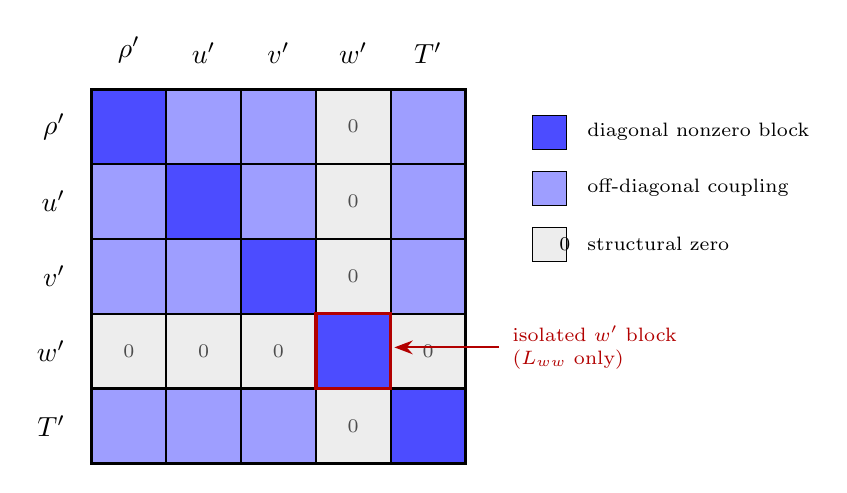
\begin{tikzpicture}[x=0.95cm,y=-0.95cm,font=\small,>=Stealth]
  \tikzset{
    nzdiag/.style={draw=black, fill=blue!70},
    nzcpl/.style={draw=black, fill=blue!38},
    zblk/.style={draw=black, fill=gray!14},
  }

  \foreach \i/\name in {0/$\rho'$,1/$u'$,2/$v'$,3/$w'$,4/$T'$} {
    \node[anchor=east,font=\bfseries] at (-0.22,\i+0.5) {\name};
    \node[anchor=south,font=\bfseries] at (\i+0.5,-0.22) {\name};
  }

  % Structural zeros implied by Eq. (block_L)
  \foreach \i/\j in {0/3,1/3,2/3,4/3,3/0,3/1,3/2,3/4} {
    \path[zblk] (\j,\i) rectangle ++(1,1);
    \node[font=\scriptsize\bfseries, text=black!70] at (\j+0.5,\i+0.5) {$0$};
  }

  % Off-diagonal nonzero couplings
  \foreach \i/\j in {
    0/1,0/2,0/4,
    1/0,1/2,1/4,
    2/0,2/1,2/4,
    4/0,4/1,4/2
  } {
    \path[nzcpl] (\j,\i) rectangle ++(1,1);
  }

  % Diagonal blocks
  \foreach \k in {0,1,2,3,4} {
    \path[nzdiag] (\k,\k) rectangle ++(1,1);
  }

  \draw[very thick] (0,0) rectangle (5,5);
  \foreach \k in {1,2,3,4} {
    \draw[thick] (0,\k) -- (5,\k);
    \draw[thick] (\k,0) -- (\k,5);
  }

  % Emphasize isolated spanwise block
  \draw[very thick, red!70!black] (3,3) rectangle (4,4);
  \draw[->, thick, red!70!black] (5.45,3.45) -- (4.05,3.45);
  \node[anchor=west, align=left, text=red!70!black, font=\scriptsize] at (5.5,3.45)
    {isolated $w'$ block\\($L_{ww}$ only)};

  % Compact legend
  \begin{scope}[shift={(5.9,0.35)}]
    \path[nzdiag] (0,0) rectangle ++(0.45,0.45);
    \node[anchor=west,font=\scriptsize] at (0.6,0.22) {diagonal nonzero block};
    \path[nzcpl] (0,0.75) rectangle ++(0.45,0.45);
    \node[anchor=west,font=\scriptsize] at (0.6,0.97) {off-diagonal coupling};
    \path[zblk] (0,1.5) rectangle ++(0.45,0.45);
    \node[anchor=west,font=\scriptsize] at (0.225,1.725) {$0$};
    \node[anchor=west,font=\scriptsize] at (0.6,1.72) {structural zero};
  \end{scope}
\end{tikzpicture}
\caption{Schematic $5\times5$ block structure of the assembled LNSE operator $\bL$ for the special case $k_z=0$. Each cell denotes an $N\times N$ sparse sub-block: dark cells are diagonal blocks, medium cells are off-diagonal couplings, and gray cells marked $0$ are structural zeros. For $k_z\neq0$, the $w'$-coupling blocks become nonzero.}
\label{fig:sparsity}
\end{figure}

\paragraph{Software architecture.}
The Python package is organized into three sub-packages:
\path{linstab2d/operators/} contains the coefficient matrices, LNSE assembly, energy-norm construction, and spatial companion linearization;
\path{linstab2d/mesh/} handles grid generation, coordinate transformations, SBP operators, and implicit filters;
\path{linstab2d/solvers/} wraps PETSc/SLEPc for linear solves, eigenvalue problems, and resolvent analysis.
A utility layer (\path{linstab2d/utils/}) provides PETSc initialization, SciPy-to-PETSc conversion, and MPI-aware matrix distribution.
Each analysis workflow (temporal, spatial, adjoint, resolvent) is exposed as a single top-level function that accepts SciPy sparse matrices and returns NumPy arrays, hiding the PETSc/SLEPc details from the caller.

%======================================================================
\section{PETSc/SLEPc solver architecture}
\label{sec:solvers}
%======================================================================

%----------------------------------------------------------------------
\subsection{Design rationale}
\label{sec:design}
%----------------------------------------------------------------------

The dominant computational cost of the analyses described in~\S\ref{sec:equations} is repeated solution of large sparse shifted non-Hermitian linear systems: $(\bL - \sigma\bM)\bx = \bb$ for eigenvalue problems and $(\bL + \mathrm{i}\omega\bM)\bx = \bb$ for resolvent analysis.
PETSc provides a unified interface for sparse matrix storage, iterative or direct linear solvers, and preconditioning, while SLEPc adds outer eigensolver and spectral-transformation layers \cite{balay2025petsc,hernandez2005slepc}.
In this section, we use PETSc/SLEPc acronyms consistently: \KSP\ (linear solver), \PC\ (preconditioner), EPS (eigenproblem solver), and ST (spectral transformation).
The assembled SciPy CSC operator is converted to a PETSc AIJ matrix once; all subsequent solves operate on the PETSc object.
This is the current default implementation path.
The target production path is direct PETSc-native distributed assembly to remove temporary SciPy storage pressure for the largest cases.

For problems exceeding the memory of a single node, the assembled operator can be distributed across MPI ranks using PETSc's row-partitioned AIJ format.
The SciPy operator is assembled on rank~0 and scattered to all ranks, after which all Krylov and direct solves execute in parallel.
The matrix distribution mode is selected automatically when \texttt{MPI\_COMM\_WORLD.size > 1}, or can be forced via the environment variable \texttt{LINSTAB2D\_PETSC\_MATRIX\_MODE}.
Figure~\ref{fig:architecture} illustrates the solver architecture and data flow.

\begin{figure}[t]
\centering
% \includegraphics[width=0.85\textwidth]{figures/architecture.pdf}
\centering
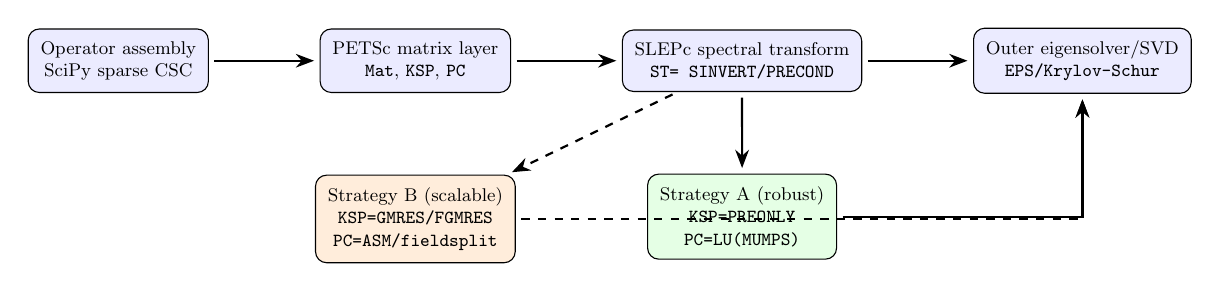
\begin{tikzpicture}[
    node distance=1.8cm and 1.9cm,
    inner sep=6pt,
    outer sep=auto,
    font=\small,
    align=center,
    scale=0.74,
    every node/.style={transform shape},
    >=Stealth,
    shorten >=2pt,
    shorten <=2pt,
    core/.style={rectangle, rounded corners, draw, minimum width=3.0cm, minimum height=1.0cm, fill=blue!8},
    patha/.style={rectangle, rounded corners, draw, minimum width=3.2cm, minimum height=1.0cm, fill=green!10},
    pathb/.style={rectangle, rounded corners, draw, minimum width=3.2cm, minimum height=1.0cm, fill=orange!14}
]
  \node[core] (asm) {Operator assembly\\SciPy sparse CSC};
  \node[core, right=of asm] (petsc) {PETSc matrix layer\\\texttt{Mat}, \texttt{KSP}, \texttt{PC}};
  \node[core, right=of petsc] (st) {SLEPc spectral transform\\\texttt{ST= SINVERT/PRECOND}};
  \node[core, right=of st] (outer) {Outer eigensolver/SVD\\\texttt{EPS/Krylov-Schur}};

  \node[patha, below=1.4cm of st] (a) {Strategy A (robust)\\\texttt{KSP=PREONLY}\\\texttt{PC=LU(MUMPS)}};
  \node[pathb, below=1.4cm of petsc] (b) {Strategy B (scalable)\\\texttt{KSP=GMRES/FGMRES}\\\texttt{PC=ASM/fieldsplit}};

  \draw[->, thick] (asm) -- (petsc);
  \draw[->, thick] (petsc) -- (st);
  \draw[->, thick] (st) -- (outer);
  \draw[->, thick] (st) -- (a);
  \draw[->, thick, dashed] (st) -- (b);
  \draw[->, thick] (a.east) -| (outer.south);
  \draw[->, thick, dashed] (b.east) -| (outer.south);
\end{tikzpicture}
\caption{Solver architecture of \texttt{linstab2d}. The SciPy CSC operator is converted to PETSc AIJ once, then all downstream operations use PETSc/SLEPc. Dashed arrows denote Strategy~B (iterative) and solid arrows denote Strategy~A (direct).}
\label{fig:architecture}
\end{figure}

%----------------------------------------------------------------------
\subsection{Strategy A: MUMPS sparse-direct}
\label{sec:mumps}
%----------------------------------------------------------------------

For non-specialist readers, the distinction is:
\begin{itemize}
\item \textbf{Direct solver:} explicitly factor the sparse matrix, then solve by forward/back substitutions.
\item \textbf{Iterative solver:} do not factor explicitly; build successive approximations using matrix-vector products and a preconditioner until the residual is below tolerance.
\end{itemize}
In this workflow, direct methods are usually more robust, while iterative methods are usually more memory-efficient.

MUMPS \cite{amestoy2001mumps} is used as the default factorization backend via PETSc's \KSP/\PC\ interface.
MUMPS is a sparse multifrontal LU solver: it uses fill-reducing reorderings, assembles dense frontal blocks, and applies partial pivoting for numerical stability.
For shift-invert eigensolves, the shifted matrix $(\bL - \sigma\bM)$ is factored once, and each outer Krylov--Schur iteration performs triangular solves with the factors.
For resolvent analysis, the MUMPS factorization of $\bL_\omega$ supports both forward and transpose solves, enabling the matrix-free application of~\eqref{eq:weighted_svd} without re-factoring.
This route is preferred when memory permits, as it is maximally robust against non-normality, difficult shifts, and aggressive boundary-penalty scaling.
Fill-reducing ordering (METIS, via MUMPS \texttt{ICNTL(7)=5}) can be activated to reduce factorization memory.
The main limitation remains fill-in growth: factor memory can become prohibitive for very large grids.

%----------------------------------------------------------------------
\subsection{Strategy B: preconditioned Krylov}
\label{sec:iterative}
%----------------------------------------------------------------------

When direct factorization exceeds available memory, a scalable iterative path is used.
For a left-preconditioned system,
\begin{equation}
  \bP^{-1}\bA\,\bx = \bP^{-1}\bb,
  \label{eq:preconditioned}
\end{equation}
Krylov iterates are built in the subspace $\mathcal{K}_m(\bP^{-1}\bA,\,\bP^{-1}\br_0)$.
For right preconditioning, one solves
\[
  \bA\bP^{-1}\by = \bb,
  \qquad
  \bx = \bP^{-1}\by,
\]
which preserves residual monitoring in the original equation space.
In \texttt{linstab2d}, the shift-invert eigenvalue inner solve defaults to left preconditioning (GMRES), while the generic iterative linear-solver path defaults to right preconditioning (FGMRES).
The former is used for robust fixed-preconditioner shift-invert iterations; the latter is used for flexible Krylov workflows where preconditioner quality may vary across iterations.
The default preconditioner is additive Schwarz (ASM) with configurable overlap, a standard domain-decomposition strategy that is robust and MPI-compatible; for readers new to this class of methods, Dolean et al.\ \cite{dolean2015introduction} is an excellent introduction.
Increasing overlap often improves convergence robustness, but also increases communication and setup cost.
For eigenvalue problems with $k_z=0$, an optional field-split preconditioner partitions the $(\rho',u',v',T')$ block from $w'$. For $k_z\neq0$, this split is heuristic rather than exact because the $w'$ equation is coupled to the remaining state variables.
This field-split option is activated via the environment variable \texttt{LINSTAB2D\_EIGEN\_PC\_TYPE=fieldsplit}.
In the current implementation, this field-split path is available for eigenvalue inner solves; resolvent inner solves remain on the ASM-based iterative route.
Compared with Strategy~A, Strategy~B reduces factor-memory pressure because no global LU factors are formed; however, robustness now depends on preconditioner quality and on the conditioning of the shifted operator.
All iterative workflows enforce strict failure semantics: a non-converged inner linear solve invalidates the outer eigensolver or resolvent result rather than being silently accepted.

\begin{table}[t]
\centering
\small
\setlength{\tabcolsep}{5pt}
\begin{tabular}{L{2.8cm}L{4.4cm}L{4.4cm}}
\toprule
Criterion & Strategy A: MUMPS sparse-direct & Strategy B: preconditioned Krylov \\
\midrule
Core mechanism & Sparse LU factorization once, then triangular solves for each right-hand side. & Iterative residual reduction with matrix-vector products and preconditioner applications. \\
Robustness & High robustness for difficult non-normal shifted systems. & Strongly dependent on preconditioner quality and shift conditioning. \\
Memory profile & Higher memory demand due to fill-in and factor storage. & Lower memory footprint (no global LU factors). \\
Setup cost & Potentially high one-time factorization cost. & Lower setup cost, but iterative convergence cost per solve. \\
Repeated solves & Efficient after factorization, especially for many solves at fixed shift. & Cost scales with iteration count; can vary across frequencies/shifts. \\
Best-use regime & Default when factors fit in memory and maximum reliability is required. & Preferred when direct factorization is memory-limited and scalable execution is needed. \\
\bottomrule
\end{tabular}
\caption{Reader-oriented comparison of direct and iterative linear-solver strategies used in \texttt{linstab2d}.}
\label{tab:direct_iterative_compare}
\end{table}

%----------------------------------------------------------------------
\subsection{Solver option summary}
\label{sec:solver_summary}
%----------------------------------------------------------------------

Table~\ref{tab:solver_rationale} summarizes the role of the main PETSc/SLEPc configuration options.

\begin{table}[t]
\centering
\footnotesize
\setlength{\tabcolsep}{4pt}
\begin{tabular}{L{1.7cm}L{2.7cm}L{2.8cm}L{3.0cm}L{3.2cm}}
\toprule
Layer & Option pattern & Default role & Why chosen & When to change \\
\midrule
SLEPc & $ST=$ SINVERT & Interior-target extraction & Maps target eigenvalues to dominant transformed eigenpairs & Change shift $\sigma$ when target region moves \\
PETSc KSP/PC & PREONLY + LU(MUMPS) & Strategy A inner solve & Maximum robustness for difficult shifted systems & Replace when factor memory becomes limiting \\
PETSc KSP/PC & GMRES + ASM & Strategy B eigensolver ST & Default iterative inner solve for shift-invert eigenproblems & Switch to fieldsplit via \path{LINSTAB2D_EIGEN_PC_TYPE} \\
PETSc KSP/PC & FGMRES + ASM & Strategy B resolvent & Flexible GMRES accommodates variable preconditioning & Adjust overlap via \path{LINSTAB2D_LINSOLVE_ASM_OVERLAP} \\
Conv. guard & \path{ksp_error_if_not_converged} & Hard failure semantics & Prevents polluted outer spectra from unconverged inner solves & Never disable for production runs \\
\bottomrule
\end{tabular}
\caption{Solver-option rationale used in \texttt{linstab2d} for large sparse shift-invert and resolvent workflows.}
\label{tab:solver_rationale}
\end{table}

All solver parameters are controlled at runtime via environment variables prefixed with \path{LINSTAB2D_}.
The main options are:
\begin{itemize}
\item \path{LINSTAB2D_LINSOLVE_TYPE} and \path{LINSTAB2D_EIGEN_ST_SOLVER}: select direct (\path{mumps}) or iterative (\path{iterative}) mode.
\item \path{*_KSP_TYPE}, \path{*_PC_TYPE}, \path{*_KSP_RTOL}, and \path{*_KSP_MAX_IT}: configure the Krylov solver and preconditioner.
\item \path{*_ASM_OVERLAP}: sets ASM overlap depth.
\item \path{LINSTAB2D_PETSC_MATRIX_MODE}: selects serial or distributed matrix assembly.
\item \path{LINSTAB2D_PETSC_SET_MUMPS_ICNTL_7}: activates METIS fill-reducing ordering.
\end{itemize}
No dedicated solver configuration file is required; solver tuning is performed through these environment variables.

\paragraph{Assembly backend and memory pressure.}
The current implementation assembles the linear operators in SciPy sparse format and then converts them to PETSc matrices for linear/eigenvalue solves.
This design was chosen during migration because it simplifies parity checks against the MATLAB reference and makes operator debugging straightforward.
However, for large refined cases it is not the ideal end state: SciPy-first assembly can temporarily duplicate sparse storage and, in root-led workflows, concentrates memory pressure before PETSc distribution.
For production-scale runs near the memory limit, the preferred architecture is direct PETSc-native assembly with distributed ownership and preallocation, so the global SciPy operator can be eliminated from the critical path.
The transition strategy is to keep SciPy assembly as a short-term parity/debug mode and make PETSc-native assembly the default path once operator-equivalence checks are complete.

%======================================================================
\section{Results}
\label{sec:results}
%======================================================================

Results are reported only for cases with archived run artifacts, frozen solver options, and recorded hardware metadata.
The main text is restricted to claim-bearing material: independent operator verification (\S\ref{sec:linearization_verification}) and Case~1 (SWBLI) solver behavior (\S\ref{sec:case1}--\S\ref{sec:scaling}).
The external-reference Martini parity audit and the associated reproducibility bookkeeping are moved to Appendix~\ref{sec:app:martini_verification}, so verification status is documented without being conflated with novelty claims.

%----------------------------------------------------------------------
\subsection{Independent verification of the linearized operator}
\label{sec:linearization_verification}
%----------------------------------------------------------------------

The coefficient matrices $\bA_k$ in~\eqref{eq:lnse_matrix} were originally derived with computer algebra (Mathematica) by M\&S, implemented in MATLAB, and then translated to Python.
Agreement with the MATLAB reference is used to confirm translation fidelity once Table~\ref{tab:accuracy_gate} is populated, but this parity check cannot detect errors shared by both implementations.
We therefore verify the assembled discrete operator $\bL$ against two independent references that do not rely on the M\&S derivation.

\paragraph{Complex-step Jacobian verification.}
The discrete nonlinear compressible Navier--Stokes residual $\bR(\bq)$ is evaluated on the same grid and with the same SBP operators used for the linearized system.
The exact Jacobian of $\bR$ at the base flow $\bqbar$ is then computed column-by-column via the complex-step method \cite{squire1998using,martins2003complex}:
\begin{equation}
  \frac{\pp R_i}{\pp q_j}\bigg|_{\bqbar}
  = \frac{\mathrm{Im}\!\left[\bR(\bqbar + \mathrm{i}\epsilon\,\mathbf{e}_j)\right]}{\epsilon},
  \label{eq:complex_step}
\end{equation}
where $\epsilon \sim 10^{-30}$ is a vanishingly small step and $\mathbf{e}_j$ is the $j$-th unit vector.
In IEEE double precision, this magnitude is far from underflow and is numerically admissible for complex-step differentiation.
Unlike finite differences, complex-step derivatives can reach near machine precision (no subtractive cancellation), provided $\bR$ is implemented without non-analytic operations (\texttt{abs}, \texttt{real}).
The resulting Jacobian matrix is compared entry-by-entry against the assembled $\bL$; discrepancies above $O(10^{-12})$ indicate coefficient errors.
For moderate grids ($n \lesssim 5000$), all $n$ columns are checked; for larger problems, a random subset of columns suffices to provide statistical confidence.

\paragraph{Symbolic re-derivation with SymPy.}
As a complementary check, the compressible Navier--Stokes equations are linearized from scratch using SymPy symbolic algebra.
The base-flow and perturbation quantities are defined as SymPy symbols; substitution of $\bq = \bqbar + \epsilon\bqp$ followed by series expansion in $\epsilon$ and collection at $O(\epsilon)$ yields the linearized equations.
The coefficient matrices $\bA_k$ are extracted by grouping terms according to the derivative operators ($D_x$, $D_y$, $D_{xx}$, etc.), and each entry is compared symbolically against the expressions implemented in \texttt{LNSECoefficients}.
This approach catches algebraic errors in the derivation itself --- including Sutherland-viscosity derivative terms, which involve second-order temperature derivatives and are particularly prone to sign or factor errors.

\paragraph{Verification status.}
This subsection defines the independent verification protocol and reporting criteria.
Before release snapshots, quantitative values are populated from automated reports, including (i) maximum relative Jacobian discrepancy from the complex-step test and (ii) symbolic agreement status for all coefficient sub-blocks.

Complete Martini parity bookkeeping is reported in Appendix~\ref{sec:app:martini_verification}.
That appendix is verification-only: it records the current state of external-reference closure for the shipped Martini examples and the commands that regenerate the audit artifacts.
The main text now turns to the Case~1 (SWBLI), which is the basis for the solver and scaling claims in this paper.

%----------------------------------------------------------------------
\subsection{Flagship large-scale case}
\label{sec:case1}
%----------------------------------------------------------------------

This subsection focuses on production-style scalability behavior on a representative large case.
The Case~1 (SWBLI) stresses the solver stack under production-scale pressure.
Both stability and resolvent workflows are reported.

\begin{table}[t]
\centering
\small
\begin{tabular}{lccccc}
\toprule
Workflow & Grid & $n = 5N$ & Leading output & Wall time [s] & Peak mem [GB] \\
\midrule
%--- Placeholder rows: populated automatically by reproducible artifact pipeline ---
Temporal EVP & $N_x \times N_y$ & pending & $\omega_1 =$ pending & pending & pending \\
Resolvent    & $N_x \times N_y$ & pending & $\sigma_1 =$ pending & pending & pending \\
\bottomrule
\end{tabular}
\caption{Case~1 (SWBLI) reporting template: leading eigenvalue and resolvent gain with solver performance under Strategy~A (MUMPS). Hardware and numerical entries are populated by the automated benchmark pipeline (see~\S\ref{sec:repro_checklist}).}
\label{tab:case1}
\end{table}

Figure~\ref{fig:case1_modes} shows the leading eigenvector and resolvent response mode for this case.

\begin{figure}[t]
\centering
\includegraphics[width=0.92\textwidth]{figs/case1_modes.png}
\caption{Case~1 (SWBLI) on the $150\times170$ grid: (a)~normalized real part of the leading temporal eigenvector component $u'$; (b)~normalized magnitude of the leading resolvent response component $|u'|$.}
\label{fig:case1_modes}
\end{figure}

%----------------------------------------------------------------------
\subsection{Runtime and memory scaling}
\label{sec:scaling}
%----------------------------------------------------------------------

Performance analysis is reported with hardware and solver metadata (MPI ranks, thread settings, linear-solver/preconditioner choices, tolerances).
Table~\ref{tab:scaling} reports wall time and peak memory as a function of problem size for Strategy~A and Strategy~B.

\begin{table}[t]
\centering
\small
\begin{tabular}{rcccccc}
\toprule
 & \multicolumn{3}{c}{Strategy A (MUMPS)} & \multicolumn{3}{c}{Strategy B (FGMRES+ASM)} \\
\cmidrule(lr){2-4}\cmidrule(lr){5-7}
$n = 5N$ & Assemble [s] & Factor [s] & Mem [GB] & Assemble [s] & Solve [s] & Mem [GB] \\
\midrule
%--- Placeholder rows: populated automatically by reproducible artifact pipeline ---
pending  & pending & pending & pending & pending & pending & pending \\
pending  & pending & pending & pending & pending & pending & pending \\
pending  & pending & pending & pending & pending & pending & pending \\
pending  & pending & pending & pending & pending & pending & pending \\
\bottomrule
\end{tabular}
\caption{Scaling reporting template: wall time and peak memory vs.\ problem size for the temporal eigenvalue problem (10 eigenvalues near shift $\sigma$). Hardware and numerical entries are populated by the automated benchmark pipeline (see~\S\ref{sec:repro_checklist}).}
\label{tab:scaling}
\end{table}

Figure~\ref{fig:scaling_plot} visualizes the scaling behavior.

\begin{figure}[t]
\centering
\includegraphics[width=0.68\textwidth]{figs/scaling_reference.png}
\caption{Heuristic reference slopes used to interpret measured scaling data: $O(n^{1.5})$ and $O(n^2)$ on a log-log axis. This figure serves as a template overlay; measured Strategy~A/Strategy~B wall times are added once the scaling table data in Table~\ref{tab:scaling} are finalized.}
\label{fig:scaling_plot}
\end{figure}

From a computational-complexity perspective, direct multifrontal factorization is robust but limited by fill-in growth as mesh refinement increases.
Iterative strategies reduce factorization memory pressure, but total time-to-solution depends on preconditioner quality and the non-normal shifted spectrum.

%======================================================================
\section{Discussion}
\label{sec:discussion}
%======================================================================

The primary engineering trade-off lies between the robustness of direct solvers and the scalability of iterative methods.
Direct MUMPS runs are reliable when memory permits.
Iterative workflows can reduce factorization memory cost but require stronger preconditioning and careful convergence diagnostics, especially for shifted non-normal systems.

Beyond solver selection, the mathematical framework documented in~\S\ref{sec:equations}--\ref{sec:discretization} enables extensions that were not straightforward in the original MATLAB implementation.
The Floquet ansatz~\eqref{eq:floquet_shift} combined with the spatial companion linearization~\eqref{eq:companion} provides spatial eigenvalues from the same operator assembly.
The Chu energy norm~\eqref{eq:chu_norm} in discretized form~\eqref{eq:W_diag} accounts for the full compressible thermodynamic coupling, and its implementation as a diagonal weight allows efficient matrix-free resolvent SVD via the MatShell interface.
The adjoint filter construction in~\S\ref{sec:filtering} preserves the formal discrete adjoint relation of the filter operator; its effect on computed gains must still be checked by filter-on/filter-off sensitivity tests.

The solver-selection workflow can be stated as a reproducible process:
\begin{enumerate}
\item assemble and validate operator blocks on the target grid;
\item run Strategy~A as the robustness reference if factor memory is feasible;
\item if factor memory is not feasible, switch to Strategy~B with ASM preconditioning (or optional field-split for eigenvalue problems) and strict convergence checks;
\item compare outputs against the Strategy~A reference on a smaller nearby case before scaling up;
\item only accept production results when inner linear solves meet the prescribed tolerances.
\end{enumerate}

\paragraph{Getting started.}
A practical first-use workflow is: (i)~install via the shipped \texttt{install.sh} script, which handles PETSc/SLEPc and all Python dependencies; (ii)~run one of the shipped validation examples to verify the solver stack against the MATLAB reference data; (iii)~reproduce a published case to build confidence in the operator assembly; and (iv)~scale up to the target configuration with Strategy~A, switching to Strategy~B only when direct factorization memory is exhausted.

\paragraph{Known limitations.}
The following limitations are documented for transparency:
\begin{itemize}[nosep]
  \item Parity-based pole closures for axisymmetric grids are currently implemented only for SBP order~2; higher orders require stencil extensions not yet available.
  \item The resolvent solver re-factors $\bL_\omega$ for each frequency $\omega_f$; no factorization cache is maintained across frequencies.
  \item The \texttt{MatShell} operator in~\eqref{eq:weighted_svd} declares a non-Hermitian problem type (\texttt{NHEP}) to SLEPc, which is conservative but may forgo Hermitian-specific solver optimizations.
  \item Field-split preconditioning is available only for the eigenvalue path, not for the resolvent linear solves.
\end{itemize}

\paragraph{Assumptions and validity range.}
\begin{itemize}[nosep]
  \item Base flow is steady and satisfies the full compressible Navier--Stokes equations to machine precision.
  \item Grid satisfies the SBP summation-by-parts property by construction.
  \item Penalty parameter $P_\mathrm{bc}=10^4$ yields boundary errors below $10^{-8}$ on the Blasius validation case.
  \item Filter strength $\alpha_\mathrm{flt}\le 0.45$ preserves the intended high-order behavior.
\end{itemize}

\paragraph{Equation-to-code map.}
Table~\ref{tab:eq_code_map} links each key equation to the implementing source file and function, so the paper serves as an annotated code walkthrough.
All paths are relative to the package root directory \path{linstab2d/}.

\begin{table}[t]
\centering
\small
\begin{tabular}{L{1.2cm}L{3.2cm}L{4.0cm}L{3.8cm}}
\toprule
Eq. & Description & File & Entry point \\
\midrule
(\ref{eq:lnse_matrix})    & LNSE matrix form           & \path{operators/coefficients.py}  & \path{LNSECoefficients}      \\
(\ref{eq:gevp})--(\ref{eq:shift_invert}) & Temporal EVP      & \path{solvers/eigenvalue.py}      & \path{temporal_eigenvalues}  \\
(\ref{eq:adjoint_op})     & Adjoint operator           & \path{solvers/eigenvalue.py}      & \path{adjoint_eigenvalues}  \\
(\ref{eq:qep})--(\ref{eq:companion}) & Spatial QEP/companion & \path{operators/spatial.py}   & \path{build_spatial_operator} \\
(\ref{eq:weighted_svd})   & Resolvent SVD              & \path{solvers/resolvent.py}       & \path{resolvent_analysis}   \\
(\ref{eq:chu_norm})--(\ref{eq:W_diag}) & Chu energy norm   & \path{operators/energy_norm.py}  & \path{build_energy_norm}   \\
(\ref{eq:floquet_shift})  & Floquet shift              & \path{operators/assembly.py}      & \path{assemble_lnse}        \\
(\ref{eq:filter_implicit})--(\ref{eq:filter_2d}) & Implicit filter & \path{mesh/filters.py}       & \path{build_filter}         \\
\bottomrule
\end{tabular}
\caption{Mapping of manuscript equations to source code entry points.}
\label{tab:eq_code_map}
\end{table}

%======================================================================
\section{Conclusions}
\label{sec:conclusions}
%======================================================================

This paper has presented both the mathematical framework and the solver architecture of \texttt{linstab2d}, an open-source Python tool for compressible linear stability and resolvent analysis.
The formulation --- compressible five-variable LNSE with Sutherland viscosity, SBP finite differences with curvilinear mapping, Chu energy-norm weighting, Floquet decomposition, spatial companion linearization, and Pad\'e implicit filtering --- is documented at the level of detail needed to reproduce or extend the implementation.
The solver layer exposes both a MUMPS sparse-direct baseline and a preconditioned iterative path; any large-DOF performance claim is restricted to the archived cases reported in Section~\ref{sec:results}.

The central contribution is the combination of mathematical transparency and solver flexibility in a single open-source package.

Several directions for future work are motivated by the known limitations documented in~\S\ref{sec:discussion}:
(i)~extending the parity-based pole closures to SBP orders higher than~2, enabling high-order axisymmetric computations;
(ii)~implementing a factorization cache across resolvent frequencies to amortize the MUMPS factorization cost when sweeping over $\omega_f$;
(iii)~declaring the \texttt{MatShell} operator in~\eqref{eq:weighted_svd} as Hermitian (\texttt{HEP}) to unlock SLEPc's Hermitian-specific solver optimizations;
(iv)~developing stronger iterative preconditioners (e.g., Schur-complement or multigrid variants) for demanding resolvent configurations;
and (v)~extending field-split preconditioning to the resolvent linear-solve path.
Broader parameter studies within the large-DOF regime and systematic comparisons with other frameworks will further establish the practical operating envelope of the tool.

%======================================================================
\appendix
\section{Verification against external references}
\label{sec:app:martini_verification}
%======================================================================

%----------------------------------------------------------------------
\subsection{Accuracy gate audit of shipped Martini exports}
\label{sec:accuracy_gate}
%----------------------------------------------------------------------

This appendix is verification-only.
It documents the current parity audit against the released Martini MATLAB exports and separates that bookkeeping from the claim-bearing Case~1 results in the main text.
The audit is regenerated by \path{linstab2d/examples/run_parity_martini.sh}, which rewrites the Python example artifacts, extracts all available MATLAB HDF5 bundles under \path{martini_examples/}, and emits \path{tools/parity/reports/martini_parity_latest.json} plus \path{tools/parity/reports/martini_parity_table.csv}.

Table~\ref{tab:accuracy_gate} summarizes the current state of closure.
At this snapshot, Example~3 is unavailable because no MATLAB export was shipped for that case, while the remaining cases are still classified as \texttt{SOFT\_FAIL}.
Accordingly, the Martini suite is used here as an audit trail and closure checklist rather than as final agreement evidence.

\begin{table}[t]
\centering
\scriptsize
\setlength{\tabcolsep}{4pt}
\begin{tabular}{L{3.0cm}L{1.8cm}L{6.0cm}c}
\toprule
Case & Scope & Primary automated audit metric & Status \\
\midrule
Example 0: curvilinear derivative & protocol & MATLAB self-check $\max|df-df_{\mathrm{an}}| = 4.09\times 10^{-4}$; current Python branch audit still fails the \texttt{x\_only} and \texttt{full\_2d} branches & \texttt{SOFT\_FAIL} \\
Example 1: Blasius resolvent & direct & $\max|\Delta \sigma| = 3.70$; leading singular value is close, but trailing gain/mode pairing is not closed & \texttt{SOFT\_FAIL} \\
Example 2: jet resolvent & direct & $\max|\Delta \sigma| = 1.31\times 10^{8}$; resolvent-gain scaling remains far from the MATLAB export & \texttt{SOFT\_FAIL} \\
Example 3: streaky boundary layer & unavailable & No corresponding MATLAB export is present in the shipped \path{martini_examples/} bundle & \texttt{UNAVAILABLE} \\
Example 4: cavity spectra/adjoints & direct & After target-based spectral matching, $\max|\Delta \omega| = 7.01\times 10^{-1}$; mode parity remains poor & \texttt{SOFT\_FAIL} \\
Example 5: paraboloid resolvent & direct & $\max|\Delta \sigma| = 2.80\times 10^{7}$; the resolvent amplification level is still far from the MATLAB export & \texttt{SOFT\_FAIL} \\
\bottomrule
\end{tabular}
\caption{Current status of the external-reference Martini parity audit, summarized from \texttt{tools/parity/reports/martini\_parity\_latest.json}. These rows are verification bookkeeping only and are not used as novelty evidence.}
\label{tab:accuracy_gate}
\end{table}

%----------------------------------------------------------------------
\subsection{Representative reference overlays}
\label{sec:resolvent_validation}
%----------------------------------------------------------------------

Figures~\ref{fig:eigenvalue_spectrum}--\ref{fig:resolvent_gains} show representative reference outputs from the Case~1 MATLAB exports.
They are kept here as qualitative diagnostics for the audit workflow.
Because the shipped Martini parity suite is not yet fully closed, these figures are not used in the main paper to support performance or correctness claims beyond the explicit audit table above.

\begin{figure}[t]
\centering
\includegraphics[width=0.68\textwidth]{figs/eigenvalue_spectrum.png}
\caption{Temporal eigenvalue spectrum for the Case~1 reference case on the complex $\omega$-plane. MATLAB exports are shown explicitly, and Python markers are overlaid when the cached run artifact is available in the local workspace.}
\label{fig:eigenvalue_spectrum}
\end{figure}

\begin{figure}[t]
\centering
\includegraphics[width=0.70\textwidth]{figs/mode_shapes.png}
\caption{Leading-mode profiles from the Case~1 MATLAB export: normalized magnitudes of $|u'|$, $|v'|$, and $|T'|$ along the wall-normal coordinate.}
\label{fig:mode_shapes}
\end{figure}

\begin{figure}[t]
\centering
\includegraphics[width=0.68\textwidth]{figs/resolvent_gains.png}
\caption{Resolvent singular values $\sigma_j$ versus mode index for the Case~1 exported configuration. MATLAB values are shown explicitly, with optional Python overlay when run artifacts are available.}
\label{fig:resolvent_gains}
\end{figure}

%----------------------------------------------------------------------
\subsection{Cross-framework comparison status}
\label{sec:cross_framework}
%----------------------------------------------------------------------

No cross-framework performance table is included at this stage.
The first requirement is closure of the external-reference Martini audit summarized in Table~\ref{tab:accuracy_gate}; without that baseline, wall-time or memory comparisons against MATLAB or other frameworks would mix implementation gaps with solver-performance effects.
Once the remaining parity mismatches are resolved, this subsection can be populated from the same report directory together with full solver and hardware metadata.

%----------------------------------------------------------------------
\subsection{Reproducibility checklist}
\label{sec:repro_checklist}
%----------------------------------------------------------------------

Two command paths are kept separate on purpose.
For the main-paper Case~1 artifacts, the current validator is
\begin{verbatim}
export LINSTAB2D_LINSOLVE_TYPE=mumps
python -m linstab2d.examples.validate_all --ref matlab_export/
\end{verbatim}
which produces \path{validation_summary.json} in the repository root.

For the external-reference Martini audit, the canonical command is
\begin{verbatim}
./linstab2d/examples/run_parity_martini.sh
\end{verbatim}
which regenerates the comparison-eligible Python example outputs, writes \path{tools/parity/martini_manifest.json}, and updates the JSON/CSV audit reports under \path{tools/parity/reports/}.

The single source of truth for the Case~1/main-results validation set remains \path{linstab2d/config/validation_cases.yaml}.
The single source of truth for the Martini audit mapping is \path{tools/parity/martini_cases.jsonc}.

\section*{Code availability}

The source code of \texttt{linstab2d} is available at:
\begin{center}
  \url{https://github.com/ricardofrantz/linstab2d}
\end{center}
The repository includes the full Python package, all validation examples with MATLAB reference data, and an automated installation script (\texttt{install.sh}) that handles PETSc, SLEPc, and Python dependencies.
The code is released under the open-source license specified in the repository root for each tagged release.
A persistent archive is deposited at Zenodo for each public release; the DOI is added to the release metadata and the camera-ready manuscript.
A fully reproducible Docker image \path{ghcr.io/ricardofrantz/linstab2d:paper} contains PETSc, validation data, and the exact scripts used to generate the reported tables and figures.

\section*{Acknowledgments}
To be completed.

\section*{Conflict of interest}
All authors declare no conflicts of interest in this paper.

\bibliographystyle{unsrtnat}
\bibliography{refs}

\end{document}
